% Use only LaTeX2e, calling the article.cls class and 12-point type.

\documentclass[12pt]{article}
\usepackage{apacite}
\usepackage{graphicx}
\usepackage{url}
\usepackage{float}


% The following parameters seem to provide a reasonable page setup.

\topmargin 0.0cm
\oddsidemargin 0.5cm
\textwidth 16cm 
\textheight 21cm
\footskip 1.0cm


%The next command sets up an environment for the abstract to your paper.




% Include your paper's title here

\title{
School Discipline and Incarceration:
An Investigation of the Real-World 
Effects of School Discipline in the American Public School System 
} 


% Author

\author{Josiah Kim}

% Include the date command, but leave its argument blank.

\date{}



%%%%%%%%%%%%%%%%% END OF PREAMBLE %%%%%%%%%%%%%%%%



\begin{document} 

% Double-space the manuscript.

\baselineskip24pt

% Make the title.

\maketitle 



% Use this for the abstract.

%\begin{sciabstract}
%  This is the abstract. 
%\end{sciabstract}



% In setting up this template for *Science* papers, we've used both
% the \section* command and the \paragraph* command for topical
% divisions.  Which you use will of course depend on the type of paper
% you're writing.  Review Articles tend to have displayed headings, for
% which \section* is more appropriate; Research Articles, when they have
% formal topical divisions at all, tend to signal them with bold text
% that runs into the paragraph, for which \paragraph* is the right
% choice.  Either way, use the asterisk (*) modifier, as shown, to
% suppress numbering.

\section*{Purpose Statement}
The purpose of this study is to investigate the relationship between school discipline and incarceration. The theory is that in terms of people, those who receive school discipline will be more likely to be incarcerated in the future than those who have not. This investigation will be conducted by the use of multiple linear regression models that relate the main independent variable(s), the different rates at which different types of school disciplinary actions are handed out (referrals, in-school suspensions, out-of-school suspensions, expulsions, and corporal punishments), to the dependent variable, incarceration rates. The multiple linear regression models will vary by lead time in hopes to uncover the time effects of the relationship between school discipline and incarceration. The control variables will include the previous year's incarceration rate, socio-economic status, and sex for public school students with ages ranging from elementary school to high school. 


\section*{Conceptualization}
There are three main concepts that are vital to this investigation. The first main concept is school discipline which can be defined as the type of school discipline handed out to students. These types of school discipline include school-related arrests, referrals to law enforcement, in-school suspensions, out-of-school suspensions, and expulsions. 

The second main concept, exclusionary school discipline, is derived from the first concept. Exclusionary school discipline is characterized as the types of school discipline that remove students from the learning environment and away from their peers. Exclusionary school discipline encapsulates out-of-school suspensions and expulsions. 

The third main concept is incarceration which is defined as incarceration post-high school.



\section*{Literature Review}
\subsection*{School Discipline and its Disparities}
The modern public school disciplinary system is a phenomena that spread through the American public schools as a means to meet the Democrat party's agenda in the 1960s. After the passage of the 1965 Elementary and Secondary Education Act, politicians quickly realized that their goals to solve poverty, unemployment and racial inequality were unrealistic. Eventually, Republicans and conservative interest groups "pushed for the introduction of market forces in public education as a necessary corrective" \cite{Moak2016}. These "punitive sanctions" which "became the cornerstone of federal education" did not come without its consequences. 

School discipline is a subject that has been widely investigated by scholars with the broad understanding that the school disciplinary system targets different groups of students disproportionately. More specifically, Black students are more than three times as likely to be suspended or expelled than their White peers \cite{Okonofua2015}. Aside from suspensions and expulsions, Black elementary school students are more than twice as likely to be referred to the office for problem behavior while Black students in middle school are more than three times as likely than their White peers \cite{Skiba2011}. Even further, Black students are over represented in corporal punishment as a form of school discipline where this form of school discipline is applicable \cite{Skiba2002}. Across the board, regardless of the type of school discipline, it is evident that Black students are disproportionately targeted by the current school disciplinary system. 

The disproportionality of the school disciplinary system targeting certain groups of students is not a new phenomena. In reality, this pattern has been consistently demonstrated towards students of color for over the last 25 years \cite{Skiba2002}. More specifically, documentation of discipline for Black male students have been consistently over-represented at all grade levels \cite{RaffaeleMendez2003}. 

Even further, the disparity in school discipline is not limited to the type of punishment either, but also the degree to which a punishment is handed out. Compared to White students, Black students tend to receive harsher school disciplinary actions which is illustrated by the fact that a Black male student is three times as likely to as likely to receive physical disciplinary penalties (corporal punishment) than their White counterparts \cite{Gregory1995}. This effect can explained, in part, by the fact that school teachers feel more troubled by infractions caused by Black students than White students while also feeling that Black students should receive harsher disciplinary actions than White students \cite{Okonofua2015}.

The creation of school discipline was deeply rooted in politics; however, its implementation impacted Black students the most creating a larger gap in racial inequality that school discipline was supposed to fix. This pattern of racial disparity is evident and consistent across the different types and degrees of school discipline being handed out to public school students. With the common understanding about the existence of widespread disparity in school discipline, a new series of investigations arose which aim to highlight the direct effect that school discipline has on students.



\subsection*{Observed Effects of School Discipline: Academic Achievement}
It is quite evident that school disciplinary actions directly impact students' academic achievement especially when it comes to out-of-school disciplinary tactics which separate students from their peers and academic facilities \cite{RaffaeleMendez2003}. Even more, when school disciplinary practices decreased by way of intervention, academic performance improved \cite{Graham2011}. Some even suggest that out-of-school suspensions systemically remove students who are academically under performing as a response to the increased accountability from schools regarding academics performance \cite{Ali2008}. Also, students who experience out-of-school suspension are more likely to either finish school late or not finish at all \cite{Mendez2002}.  

School disciplinary practices that take students away from the academic environment and their peers lead to a decrease in academic achievement in terms of test scores and dropout rates. Similar to the disparity in school discipline, there is also common pattern with regards to the disparity in academic achievement between Black and White students as well, namely, the Racial-Achievement gap \cite{Lee2002}. 



\subsection*{Observed Effect of School Discipline: Juvenile Exposure to the Justice System}
Many suggest exposure to the justice system to be closely related to school disciplinary actions. School discipline can lay a path toward incarceration while also contributing to school failure \cite{Okonofua2015}. Out-of-school suspension takes students out of the classroom and places them at home, unsupervised, which gives these students a greater opportunity to commit juvenile crimes exposing them to the justice system at a young age \cite{Jacob2003}. 

As if the overwhelming evidence of disparity in school disciplinary practices was not enough, modern zero tolerance policies (e.g., exclusionary disciplinary practices which include out-of-school suspension and expulsion) have led students to face the justice system as juveniles. More specifically, many students who face suspension are immediately referred to juvenile justice agencies where they are treated as criminals with the possibility of ending up in secure detention facilities. This process is widely known as the "School-to-Prison Pipeline" which also disproportionately affects Black students as well \cite{Schiff2013}.  

The school-to-prison pipeline is discussed by many scholars, but definitions of this process varies. However, the various definitions have similar characteristics in the sense that they operate with some basic underlying assumptions: 
\begin{itemize}
  \item exclusionary school discipline is widespread, systemic, and increasing, 
  \item exclusionary school discipline increases the probability for juvenile justice involvement,
  \item the process affects some population, disproportionately, and 
  \item there is a direction of causality which starts with the policies and practices of the school \cite{Skiba2014}. 
\end{itemize}

Public schools have been increasingly referring students to police and juvenile justice systems even when the infraction is relatively minor \cite{Wilson2014}. Shocking, though, is the fact that the United States has the largest juvenile corrections rate in the world while also being five times higher than the next highest country \cite{Aizer2015}. Black students are at a disproportionate risk for exclusionary school discipline; therefore, the school-to-prison pipeline affects Black students disproportionately than another other group of students \cite{Skiba2014}. Even more, when looking at the populations of prisons and juvenile justice centers, most individuals were victims of the school-to-prison pipeline \cite{Wald2003}. 



\section*{Operationalization}
Each concept of this investigation can be operationalized for the purposes of analysis. School discipline can be operationalized as the proportion of students who have received school discipline. Then, incarceration can be defined as the number of people who have been admitted into state prison. 



\section*{Overview and Hypothesis}
The above sections exemplify the disparity placed upon Black students because and as a result of primary and secondary school disciplinary practices. Black students are disproportionately targeted by disciplinary practices with regards to the type and degree of punishment handed out which disproportionately affects Black students' level of academic achievement which disproportionately exposes this group of students to the justice system as juveniles. 

Among many other effects of school discipline, incarceration is one that has been investigated thoroughly in the juvenile context with little research done post-secondary education. One related study suggests that exclusionary school disciplinary practices is a significant indicator for later incarceration among women \cite{William2001}. However, this study focused solely on female students. Another study suggests that students are more at risk for juvenile incarceration if they are a victim of exclusionary school discipline \cite{Monahan2014}. However, incarceration later-on was not taken into account in the study.

These disparities regarding the school discipline system and the current disparities within the criminal justice system lead me to believe that school discipline may be a significant indicator for future incarceration. 

My general theory is that those groups of students who have received school discipline will be more likely to be incarcerated later-on. More specifically, I expect that exclusionary school discipline (out-of-school suspensions, expulsions with educational services, expulsions without educational services) to be significant predictors for later incarceration. 

The following are my hypotheses:

\begin{center}
  \emph{H1: Exclusionary school discipline is a 
  \newline significant predictor of later incarceration.}

  \emph{H2: Out-of-school suspension is a 
  \newline significant predictor of later incarceration.}

  \emph{H3: In-school suspension is a 
  \newline significant predictor of later incarceration.}

  \emph{H4: School-related arrests is a 
  \newline significant predictor of later incarceration.}

  \emph{H5: Expulsion without educational services 
  \newline is a significant predictor of later incarceration.}

  \emph{H6: Expulsion with educational services 
  \newline is a significant predictor of later incarceration.}

  \emph{H7: Corporal punishment is a 
  \newline significant predictor of later incarceration.}
\end{center}



\section*{Population and Sampling}
The main approach to this investigation is to "follow" a group of students from high school into adulthood (post-high school) to hopefully observe the direct effect of school discipline on incarceration. From the raw data sources, we have two entirely different populations of individuals. One population is all the inmates admitted into state prisons while the other is all public school students. The goal is to isolate the intersect between these two populations. 

From the population of all public school students, the sample will contain all students attending high school between the years 2013 and 2014. On the other hand, from the population of all inmates admitted into state prisons, the sample will contain inmates admitted into prison between the years 2015 and 2019. 



\section*{Data and Measurement}
For this analysis, I draw from two datasets sourced from two data sources. The two data sources include the Civil Right Data Collection (CRDC) and National Corrections Reporting Program (NCRP). The CRDC data is measured at the school-level and the NCRP data is measured at the inmate-level. For the purpose of this analysis, the datasets are merged. 

The Office of Civil Rights (OCR) uses data from the CRDC to ensure equal access to education and enforce civil rights in public schools. CRDC includes data about enrollment, preschool, math and science courses, AP, SAT \& ACT, student retention, harassment or bullying, discipline, restraint or seclusion, school staff, and school expenditures. All public schools are required to report this information every school year. The NCRP data is used to monitor the nation's correctional population and address specific policy questions related to recidivism, prisoner reentry, and trends in demographic characteristics of the incarcerated and community supervision populations. All persons admitted to state prison, released from state prison, or in state prison at year-end. 

I will be first be using the CRDC's \emph{enrollment} (N=95,597) and school discipline datasets for the 2013-2014 school year. The school discipline dataset is divided into nine different sub-datasets which include: \emph{corporal punishment} (N=95,597), \emph{in-school suspension} (N=95,597), \emph{a single out-of-school suspension} (N=95,597), \emph{more than one out-of-school suspensions} (N=95,597), \emph{referrals to law enforcement} (N=95,597), arrests (N=95,597), \emph{expulsions without educational services} (N=95,597), \emph{expulsions with educational services} (N=95,597), and \emph{expulsions under zero tolerance policies} (N=95,597). The last dataset I will be employing is NCRP's \emph{Prison Admissions} (N=16,936,069) dataset for the years 1991 to 2019.   

My main outcome variable of interest is the number of inmates admitted into state prisons between 2015 and 2019 (\emph{inmate\_admission\_count}). Some of the main independent variables I am interested in are the proportion of high school students who receive corporal punishment (\emph{corp\_prop}), the proportion of high school students who receive in-school suspension (\emph{iss\_prop}), the proportion of high school students who receive a single out-of-school suspension (\emph{single\_oos\_prop}), the proportion of high school students who receive more than one out-of-school suspensions (\emph{multiple\_oos\_prop}), the proportion of high school students who receive expulsion without educational services (\emph{exp\_woe\_prop}), the proportion of high school students who receive expulsion with educational services (\emph{exp\_we\_prop}), the proportion of students who receive expulsion due to zero tolerance policies (\emph{exp\_zero\_prop}), the proportion of students referred to law enforcement (\emph{ref\_prop}), and the proportion of students arrested due to school-related incidents (\emph{arr\_prop}).


\section*{Analysis and Findings}
Since I am employing school discipline data for the 2013-2014 school year, I am limited to analyzing inmate admission data between 2015 and 2019. After filtering out the NCRP data for inmates admitted before 2014, I filtered out the entries of inmates who did not graduate high school or receive a GED (education $\ne$ 2). Then, I merged this reduced dataset with the CRDC dataset. 


Figure \ref{fig:crdc} shows the proportion of students who receive school discipline by state. For the purpose of this graphic, the proportion is calculated by pooling together the different types of school discipline. At first glace, its hard to see any patterns. However, if my intuition is correct we should see this graph to be somewhat similar to the distribution of state prison admissions by state in figure \ref{fig:ncrp}.

\begin{figure}[H]
  \centering
  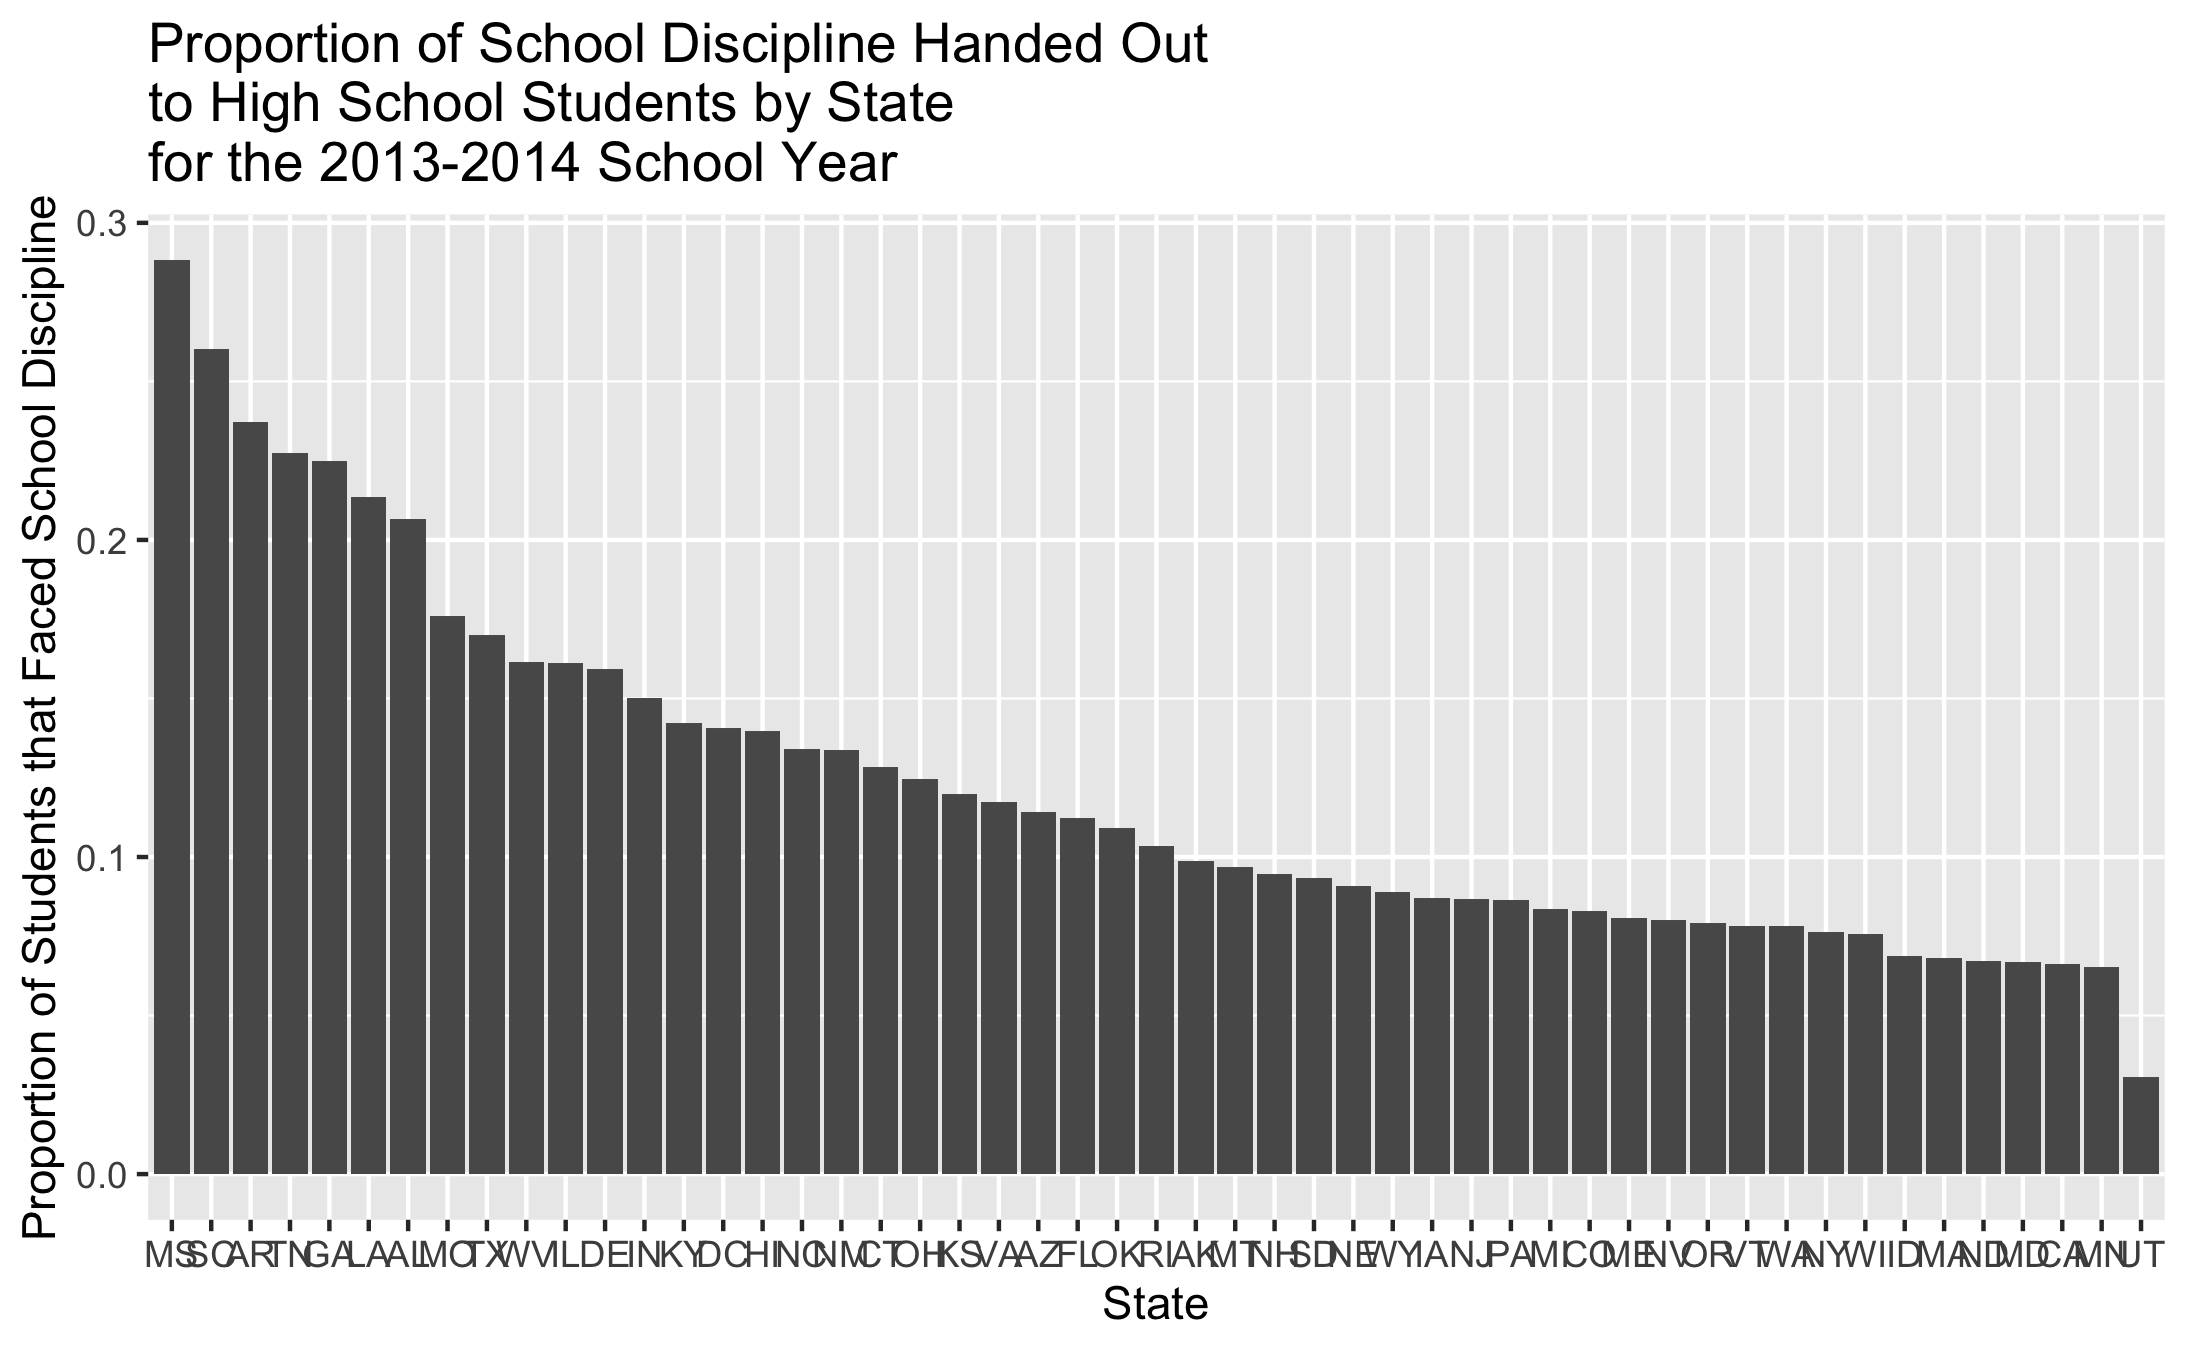
\includegraphics[width = 12cm]{CRDC_bar.png}
  \caption{Proportion of School Discipline}
  \label{fig:crdc}
\end{figure}

In figure \ref{fig:ncrp}, we can see that the distribution for state prison admissions is slightly similar to figure \ref{fig:crdc}. The states with the largest proportion of high school students who were subject to school discipline are generally the same state that have the most state prison admissions. While there is a clear outlier, Texas, my observation still stands. Another pattern that I see in figure \ref{fig:ncrp}, is that the largest states, regarding population, have the most prison admissions. 

\begin{figure}[H]
  \centering
  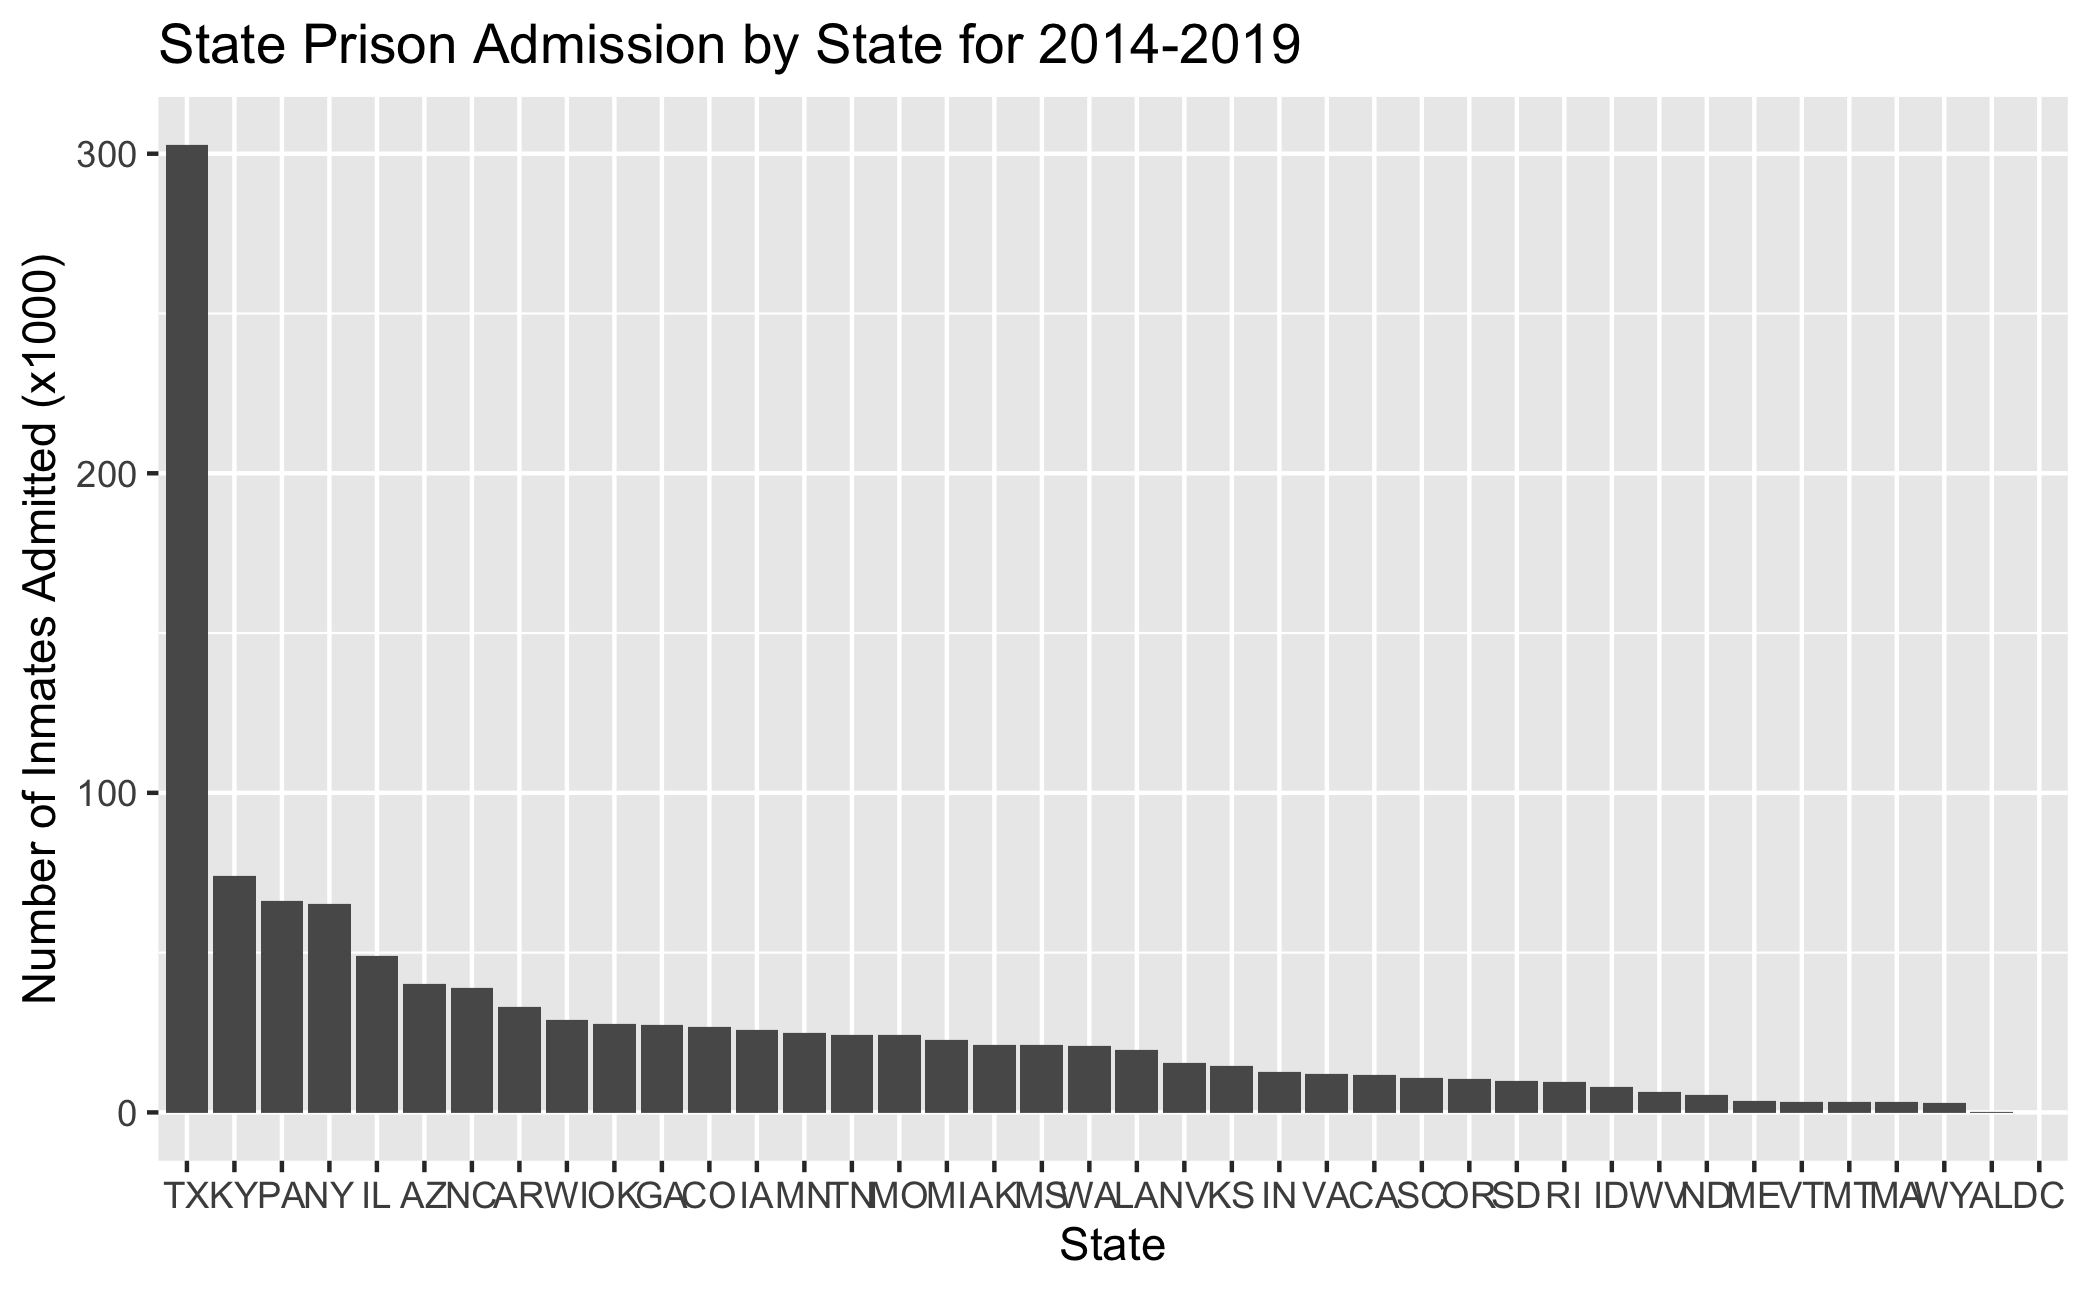
\includegraphics[width = 12cm]{NCRP_bar.png}
  \caption{Prison Admissions}
  \label{fig:ncrp}
\end{figure}

Figure \ref{fig:corr} shows a correlation matrix using the pearson's \emph{r} metric between all of my main independent and dependent variables. The matrix uncovers some interesting interactions: 
\begin{itemize}
  \item the proportion of high school students that have received corporal punishment, in-school suspensions, a single out-of-school suspension, expulsions with educational services, and school-related arrests are moderately positively associated with the number of inmates admitted into state prison,
  \item the proportion of high school students that have received multiple out-of-school suspensions, expulsions without educational services, and expulsions under zero tolerance policies are moderately negatively associated with the number of inmates admitted into state prison,
  \item the proportion of high school students that have received suspensions is strongly positively associated with expulsions,
  \item and the control variables, school-level diversity index and state population, is strongly positively associated with the the number of inmates admitted into state prison.
\end{itemize}


\begin{figure}[H]
  \centering
  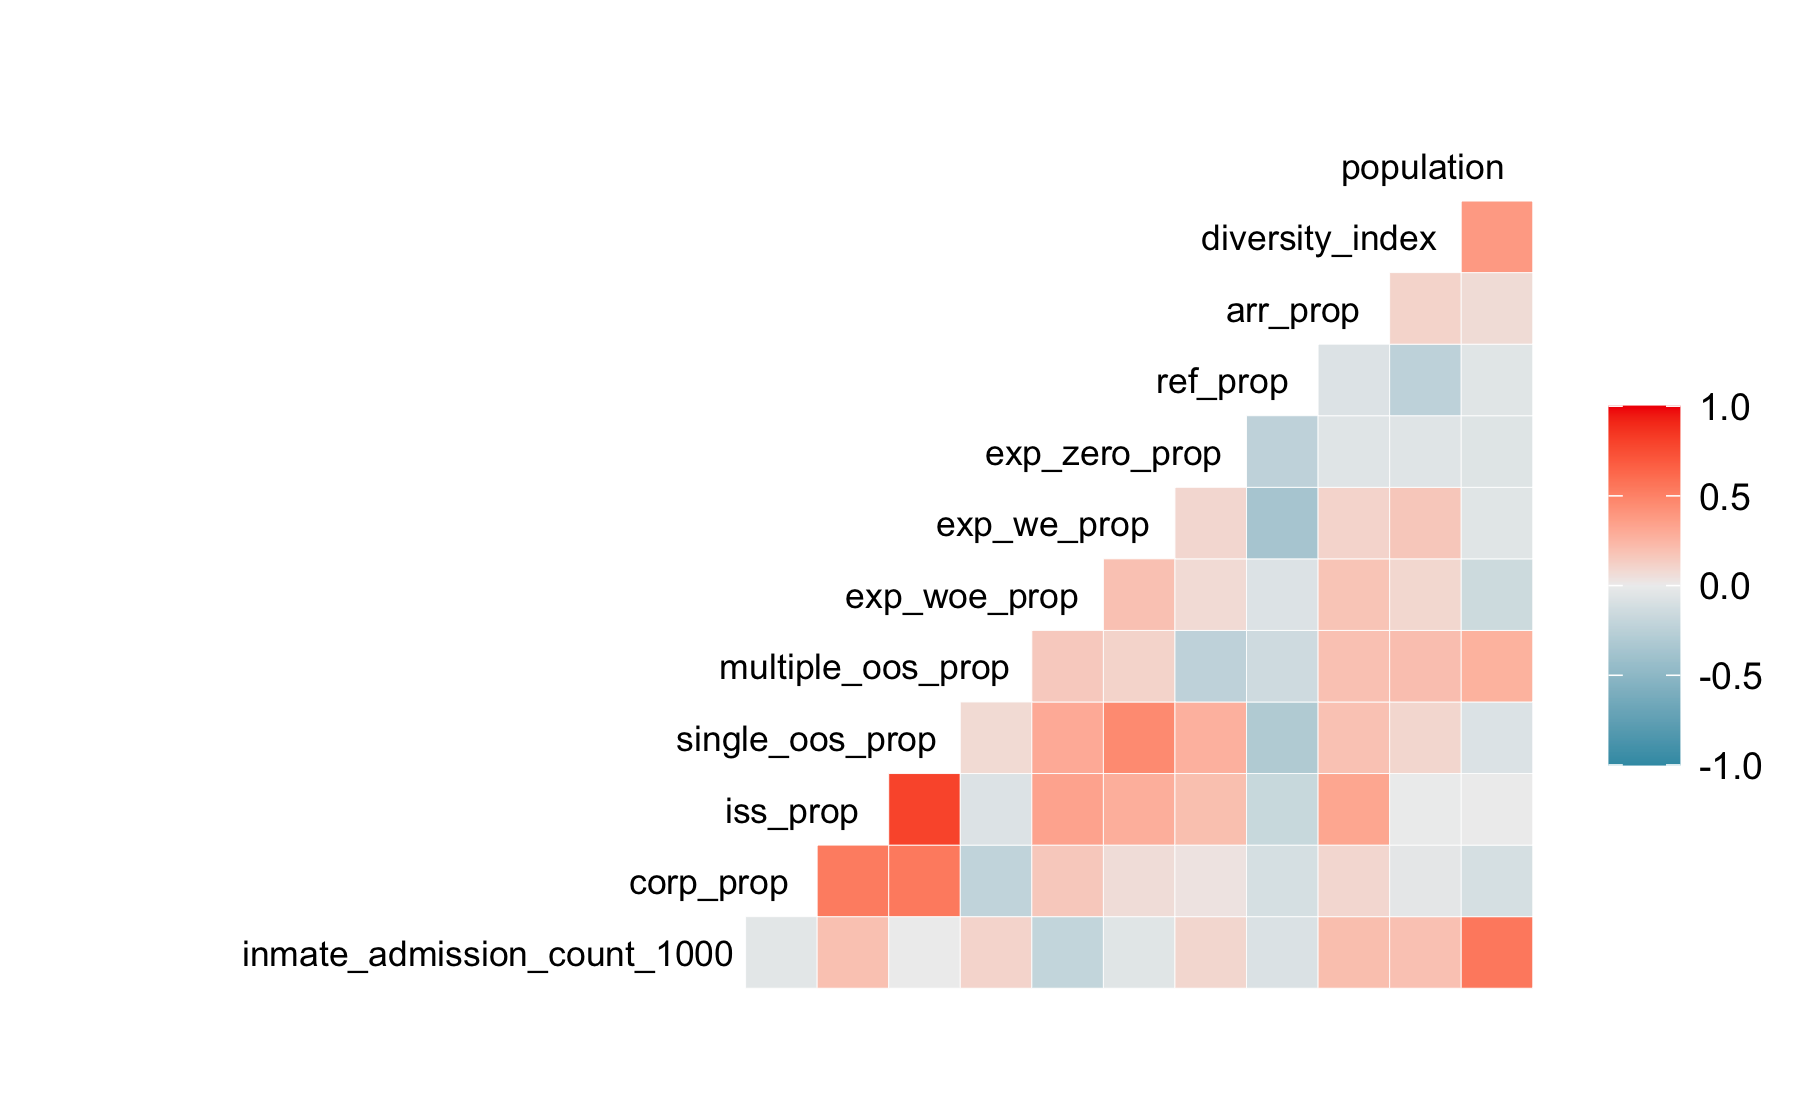
\includegraphics[width = 17cm]{corMatrix.png}
  \caption{Correlation Matrix}
  \label{fig:corr}
\end{figure}

Looking at the analysis in figure \ref{fig:ols}, I can reject the following hypotheses: H1, H2, H4, H5, H6, and H7. Hypothesis H2 still remains a valid assumption since the proportion of high school students that receive in-school suspension is a significant predictor for the number of inmates admitted into state prison. The other significant predictor for the number of inmates admitted into state prison is state population, a control variable.

\begin{figure}[H]
  \centering
  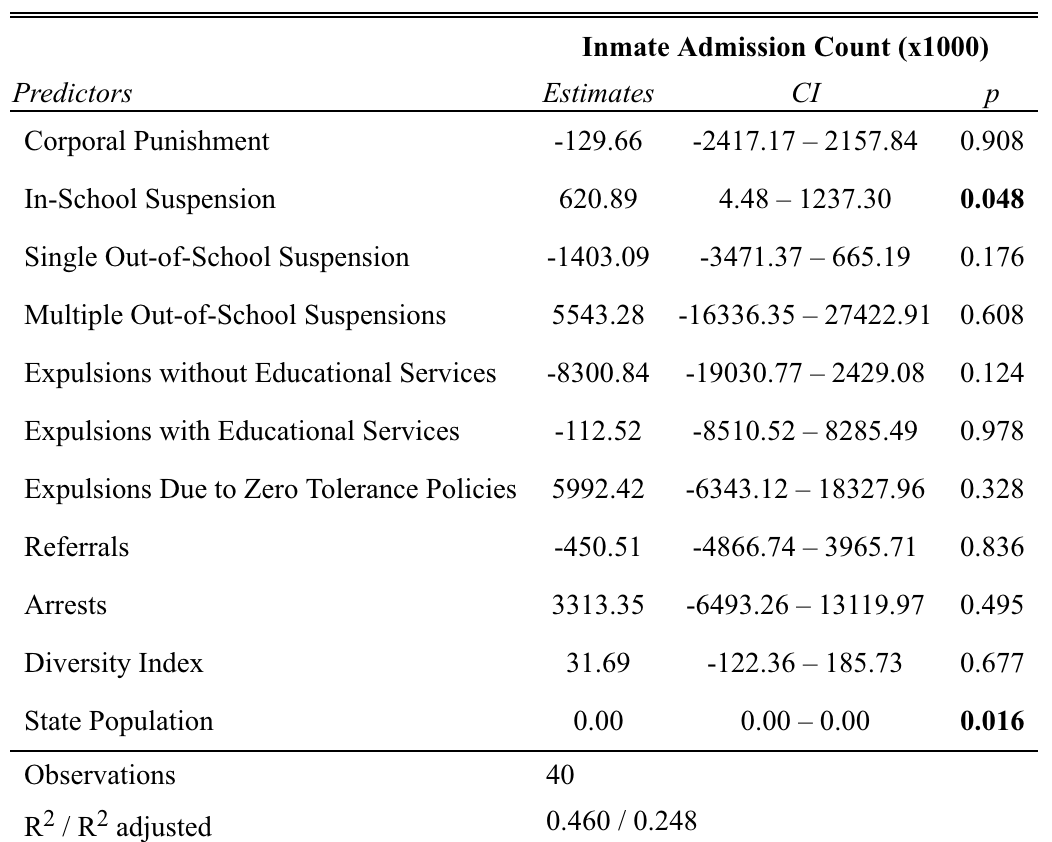
\includegraphics[width = 17cm]{ols.png}
  \caption{OLS Model}
  \label{fig:ols}
\end{figure}

\clearpage

\section*{Summary and Discussion}
It was surprising to see that more of the independent variables were not statistically significant which resulted in the rejection of the majority of my hypotheses. However, the proportion of students who received in-school suspension was a statistically significant predictor of state prison admission which leads us to believe that, although not conclusive, groups of students who receive in-school suspension are more likely to be incarcerated later-on. This is an important finding that is consistent with my literature review. Establishing that Black students are more likely to receive suspensions than they white peers, this finding supports the idea that in-school suspension could be a causal mechanism of later incarceration - feeding the disparity of Black Americans who are incarcerated.

It is important to note the restrictions placed upon my analyses due to the differences in measurement of the data sources. To be specific,the NCRP dataset is measured at the inmate (individual) level while the CRDC dataset is measured at the school-level. Due to this constraint, I had to reduce all the datasets to the state-level diminishing the granularity of the datasets, greatly. As a result, I was not able to separate out each grade in high school which would have more accurately represented the population I am trying to study. Ideally, the sample of public school students would contain all high school students in their final year (seniors) between the years 2013 and 2014. This sample would assure that we are observing our specified population with the least amount of error. 

Some other weaknesses of my analyses stem from data constraints as well. This includes the fact that this investigation only accounts for the treatment of school discipline to high school students and assumes that those students who received school discipline remain in the same state as their high school post-graduation. 

A control variable I included in my analyses was measure for school-level diversity index. This variable was calculated from the CRDC's enrollment database with reference to the USA Today Index of Ethnic Diversity Equation (Figure \ref{fig:DI}) which is commonly used by the US Census to show ethnic diversity in a region of the country. I included diversity index as a control variable because school discipline is an indicator of how criminals are disciplined in the real-world and school diversity is an indicator of how schools discipline students \cite{Moak2016}.  

\begin{figure}[H]
  \centering
  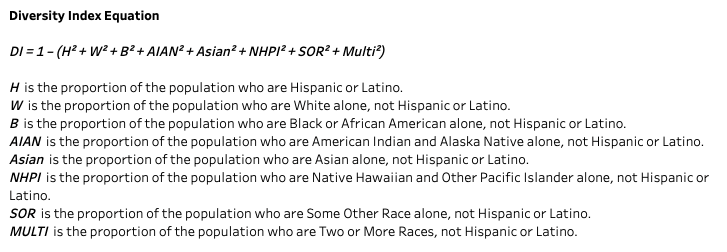
\includegraphics[width = 17cm]{DiversityIndex.png}
  \caption{Diversity Index Equation}
  \label{fig:DI}
\end{figure}

Another control variable I included was state population. I noticed that the largest states (by population) had the most inmates admitted into state prisons which indicated that it may be a confounding factor in the interaction that I was observing.

This investigation can be improved with the employment of a more granular school discipline database. The addition of more control variables may also lead to an improvement in this investigation as we are studying a complex relationship with many possible confounders. I also believe that a larger, more complex, inmate admission database that includes federal prisons and demographic information about inmates may lead to improvements in our analyses as well. 

\clearpage


\bibliographystyle{apacite}
\bibliography{references}





% Following is a new environment, {scilastnote}, that's defined in the
% preamble and that allows authors to add a reference at the end of the
% list that's not signaled in the text; such references are used in
% *Science* for acknowledgments of funding, help, etc.



\end{document}




















